\documentclass{article}
\usepackage[utf8]{inputenc}

\title{A Study of Linkages and Configuration Spaces}
\author{Evan Harwin}
\date{March 2020}

\usepackage{amssymb}
\usepackage{amsmath}
\usepackage{natbib}
\usepackage{graphicx}

\begin{document}

\maketitle

\section{Introduction}
\subsection{Abstract}
\subsection{Definitions}

\subsubsection{Planar Linkages}

This project will look at structures known as planar linkages. These are composed of a simple, connected and finite graph $L$ paired with a length function $\ell: E(L) \rarr \mathbb R^+$. The notation $(L,\ell)$ denotes this linkage. \\\\ These linkages should be intuitively thought of as a series of rigid rods in the real plane (the reader is free to consider $\mathbb C$ or $\mathbb R^2$, in this report we shall consider it $\mathbb R^2$), joined with rotating joints at the ends. This project shall ignore the possibility of constraints on movement of this linkage brought about by collision of these rods.

\begin{figure}[h!]
\centering
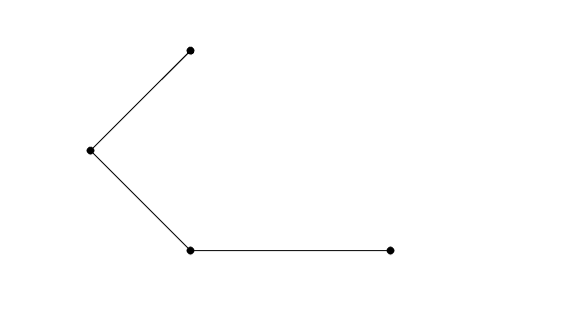
\includegraphics[scale=0.5]{./images/2-arm}
\caption{A Planar Linkage}
\label{fig:A Planar Linkage}
\end{figure}

\subsubsection{Configuration Spaces}

The way we shall relate these linkages to topological objects is through the notion of a configuration space (sometimes called a moduli space in other literature on the topic). The idea behind this is to look at the unique states that our linkage can be manipulated into. \\\\ The notion of closeness in our configuration space comes from making small adjustments to the angles subtended from the rods in our linkages. \\\\ The configuration space $M$ of a linkage $(L,\ell )$ with $|E(L)| = n$ shall be defined as follows:
$$ M(L,\ell) := \{(\boldsymbol\alpha_1,..., \boldsymbol\alpha_n) \in (\mathbb S^1)^n | \textrm{ for any cycle } l_i, ..., l_j \in L: \sum_{k=i}^j \boldsymbol\alpha_k \ell_k = 0 \} / SO(2)$$
Put more intuitively, we are defining our configuration space to be the set composed of $n$ length arrays such that the $n$-th value in this array is an angle (given by a length one vector in $\mathbb R^2$ or equivalently, a value in $\mathbb S^1$) that describes the position of the $n$-th link. We then have the constraint that any cycle in $L$ has to be such that the series of links start and end in the same position in the plane (as such the sum of the directed lengths is zero). Finally we note that we are not interested in any transformation that corresponds to 'moving' our linkage around in the plane, and as such we take this space modulo all orientation preserving isometries in 2 dimensions ($SO(2)$). \\\\ This way of defining a configuration space is in line with the work done by Kevin Walker \cite{kevinwalker}, although, as shown in his paper it turns out to be the same as other methods used elsewhere. The way to think about this is that we are taking one link in our linkage and fixing it in place, and the considering possible states that all of the other links could take.

\subsection{Motivation}

\subsubsection{Applications of Linkages in Robotics and Manufacturing}

Many things in engineering can be modelled as linkages, but one simple example that may help as a mental model is the robot arm. The linkages we look at here can, and often are, be made with fixed length rods with motorised joints that can then manipulate objects in a manifacturing line. \\\\ One example of this is pick and place machines (figure \ref{Pick and Place Machine}), used to place components into printed circuit boards to be soldered by other machines.

\begin{figure}[h!]
\centering
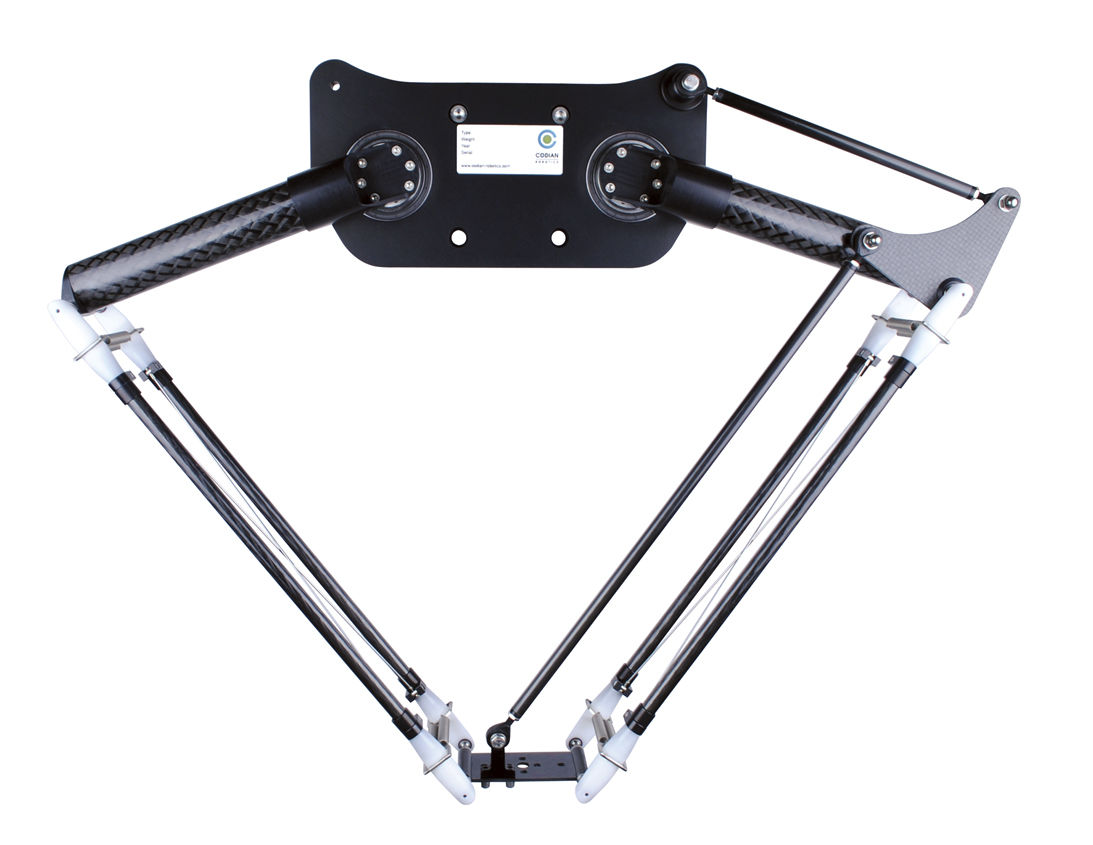
\includegraphics[scale=0.5]{./images/two_axis_pick_and_place.jpg}
\caption{A Pick and Place Machine.}
\label{fig:Pick and Place Machine}
\end{figure}

\subsubsection{What We Can Hope to Learn About Linkages From Topology}
If we understand the topological space representing the positions of our linkage we can map out 
\subsubsection{What We Can Hope to Learn About Topology From Linkages}

\section{Finding The Configuration Space of A Planar Linkage}

\subsection{Basic Idea}

The first problem to tackle is to confirm we know how to find the configuration space of a planar linkage. This will lead to intuition on the nature of configuration spaces, as well as giving us some ways to describe different states of a linkage.

\subsection{Examples}

\subsubsection{The 2-Arm}

\begin{figure}[h!]
\centering
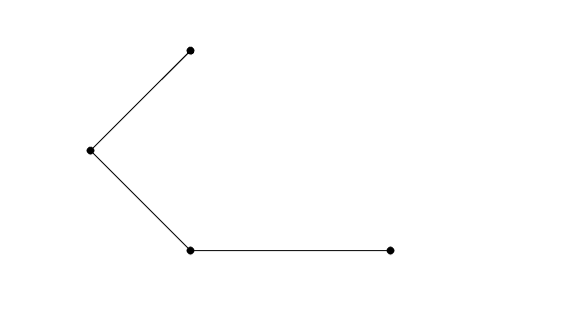
\includegraphics[scale=0.5]{./images/2-arm}
\caption{The 2-Arm}
\label{fig:The 2-Arm}
\end{figure}

\noindent The 2-Arm is one of the most simple linkages we can build, and working out its configuration space is no challenge. We can see that it has two links that are free to move in the plane, connected on the left hand side of the base. As such we need two angles to record the position of this structure, leading us to a configuration space of $\mathbb S^1 \times \mathbb S^1 \simeq T^2$.

\begin{figure}[h!]
\centering
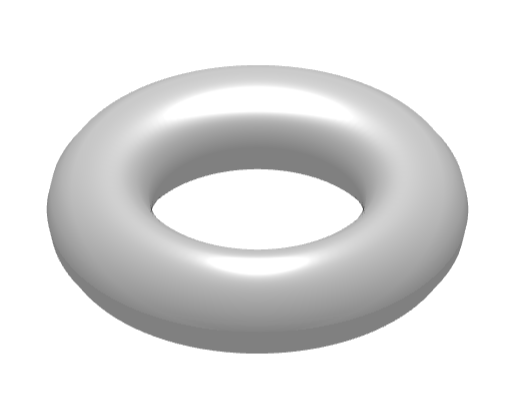
\includegraphics[scale=0.5]{./images/torus}
\caption{A Torus, The Configuration Space of The 2-Arm}
\label{fig:A Torus, The Configuration Space of The 2-Arm}
\end{figure}

\noindent This means that any state that we can put this linkage into can be uniquely identified with a position on the surface of a torus. It is not hard to see that this argument can then be generalised to stating an $n$-Arm having a configuration space of $\underbrace{ \mathbb S^1 \times \dots \times \mathbb S^1}_\text{n times} \simeq$ the $n$-dimensional torus ($T^n$). \\\\ In fact, this happens to be the case for any tree graph $L$ (no cycles) paired with any length function $\ell$ as all of the links are free to move in full circles, and none of the ends of the links have to intersect.


\subsubsection{The Triangle}

\begin{figure}[h!]
\centering
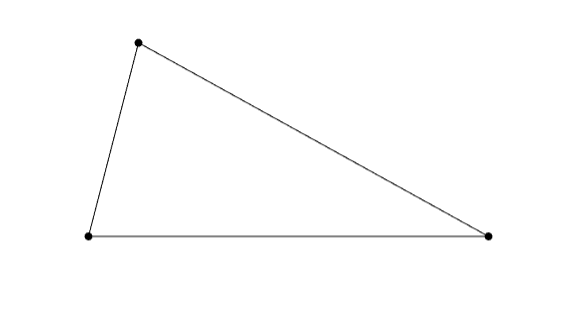
\includegraphics[scale=0.5]{./images/triangle}
\caption{The Triangle}
\label{fig:The Triangle}
\end{figure}

\noindent The triangle is the most basic linkage that we can look at to demonstrate the interesting properties that come with cycles in our linkage. In this case it might be hard to see any way this linkage could be modified without changing the lengths of the sides, and in a sense this is valid. This is as there are no topologically 'close' states that we can move this into. However, there are (if the lengths of the sides are as shown in figure \ref{fig:The Triangle}) two states that this can be in, as shown in figure \ref{fig:The Alternate Position of The Triangle}. 

\begin{figure}[h!]
\centering
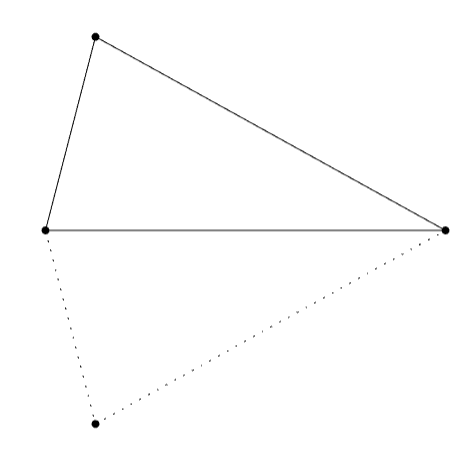
\includegraphics[scale=0.5]{./images/triangle_alt_switch}
\caption{The Alternate Position of The Triangle}
\label{fig:The Alternate Position of The Triangle}
\end{figure}

\noindent As there is no way we can transform this from one of the states into the other by continuously changing the angles of the links, we can tell we have a configuration space composed of two disjoint points, i.e. $\mathbb S^0$. \\\\ However, this result is also dependant on the length function on our graph. We can see that if the length of the base is as long as the other two links then the two disjoint positions collapse into one, as shown in figure \ref{fig:The Alternate Position of The Triangle Fixed}.

\begin{figure}[h!]
\centering
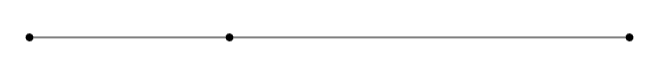
\includegraphics[scale=0.5]{./images/triangle_alt_switch_fixed}
\caption{The Alternate Position of The Triangle Fixed by $\ell$}
\label{fig:The Alternate Position of The Triangle Fixed}
\end{figure}

\noindent Hence, we have to specify the lengths of the sides to get our configuration space. Looking at a graph $L$ with edges $e_1,e_2,e_3$ such that $e_1$ is the base, we have:
$$
M((L,\ell)) = 
\begin{cases}
\mathbb S^0 \text{ if } \ell(e_1) < \ell(e_2) + \ell(e_3) \\
\mathbb * \text{ if } \ell(e_1) = \ell(e_2) + \ell(e_3) \\
\mathbb \varnothing \text{ if } \ell(e_1) > \ell(e_2) + \ell(e_3) \\
\end{cases}
$$

\begin{figure}[h!]
\centering
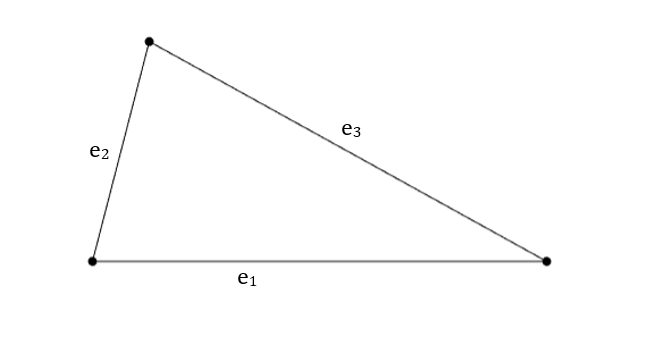
\includegraphics[scale=0.5]{./images/triangle_labeled.png}
\caption{Labeled Triangle}
\label{fig:Triangle Labeled}
\end{figure}

\noindent This structure given by the triangle, with two points a fixed length apart and two links in between them turns out to be a fairly powerful idea, as it can provide disjointedness in the configuration space in a way that proves useful. For this reason it seems sensible to highlight the key points. We shall call this a 'switch' and in all cases we're interested in it shall have three states: the two disjoint positions that it takes when the fixed length is sufficiently short, and the position it has when the two positions are identified as the fixed length is the same length as the sum of the two links.

\subsubsection{The Rectangle}

This is a natural extension from the triangle and again gives us some more ideas to work with. The manifold that this provides as a configuration space once again hugely depends on the lengths. However we shall look at a single case: The graph we are interested in is, a 4-cycle ($C_4$) and the length function we want to look at gives us a rectangular shaped linkage. We want opposite sides to have the same length, but we don't want all sides to have the same length, so we impose the constraint that adjacent edges have different lengths and denote this length function with the array $[a,b,a,b]$.

\begin{figure}[h!]
\centering
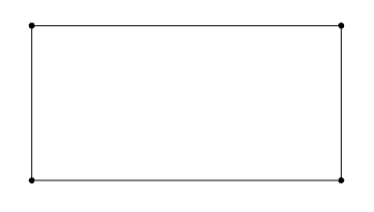
\includegraphics[scale=0.5]{./images/rectangle.png} 
\caption{The Rectangle Linkage: $(C_4, [a,b,a,b])$}
\label{fig:The Rectangle Linkage}
\end{figure}

\noindent We can see (in figure \ref{fig:Rectangle Skewed}) that the first link is free to move about all angles.

\begin{figure}[h!]
\centering
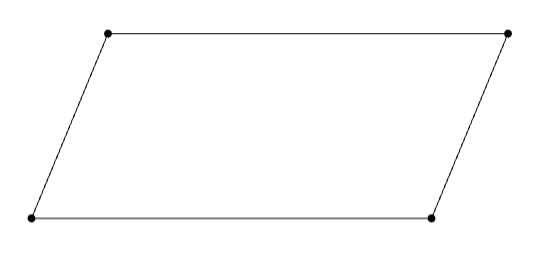
\includegraphics[scale=0.4]{./images/rectangle_skewed.png}
\caption{Freedom in the first link}
\label{fig:Rectangle Skewed}
\end{figure}

\noindent We can also note that this construction has a switch (shown in figure \ref{fig:The Rectangle Switch}) formed of the top and rightmost link between the ends of the fixed base and the free leftmost link. \\\\ An observation to make here is that we are free to order the links as we wish when describing their positions. An easy way to argue this is to note that if we consider the displacement of the end vertex when looking at the links in order we are adding vectors in $\mathbb R^2$ with the requirement that we get back to the origin. However, vector addition in $\mathbb R^2$ is commutative, implying that the order is inconsequential. \noindent \\\\ We can see that $M((C_4,[a,b,a,b]))$ is going to be something involving $\mathbb S^1$ as there is a free angle. However, we're looking at a disjoint pair of them, due to the disjoint switch positions. This linkage allows us to collapse the two disjoint switch positions into one, when the leftmost link is parallel to the fixed base, pointing to the left (figure \ref{fig:Rectangle Flat}). The meaning that this has on the configuration space is that it identifies our pair of disjoint $\mathbb S^1$'s at a single point, giving us: $M((C_4,[a,b,a,b])) \simeq \bigwedge_2 \mathbb S^1$ (the wedge product of two circles).

\begin{figure}[h!]
\centering
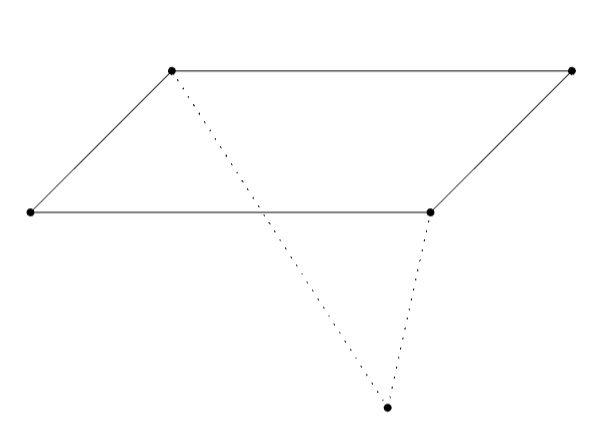
\includegraphics[scale=0.4]{./images/rectangle_skewed_alt_switch.png}
\caption{The Switch In The Rectangle}
\label{fig:The Rectangle Switch}
\end{figure}



\begin{figure}[h!]
\centering
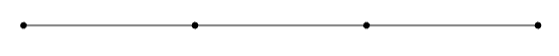
\includegraphics[scale=0.4]{./images/rectangle_flat.png}
\caption{The Switch In The Rectangle, Fixed to One Position}
\label{fig:Rectangle Flat}
\end{figure}

\subsection{Homotopies Between Configuration Spaces and Manifolds}

\subsubsection{Idea}

So we have the concept of identifying a state of a linkage with a position on a manifold, and with some hand waving, we can get an idea of what that manifold will look like. However, it would be good to pin down this idea with some more rigour and describe the homotopy in a way that makes it more convincing.

\subsubsection{Graphical Intuition}

We can look to the 2-arm as an example. The argument we made was that the configuration space had to be equivalent to a torus as the position of the linkage could be described by two angles, we'll call them $\alpha_1$ and $\alpha_2$ (see figure \ref{fig:2-arm Labeled Angles}).

\begin{figure}[h!]
\centering
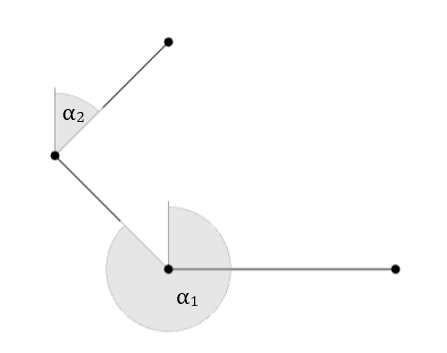
\includegraphics[scale=0.4]{./images/2_arm_labeled_angles.png}
\caption{Identifying the Positions of the 2-arm}
\label{fig:2-arm Labeled Angles}
\end{figure}

\noindent Now, the key is that this can also be used to identify a point on the torus. (see figure \ref{fig:Torus Labeled Angles}). This means we can define a bijective and invertable map between the two.

\begin{figure}[h!]
\centering
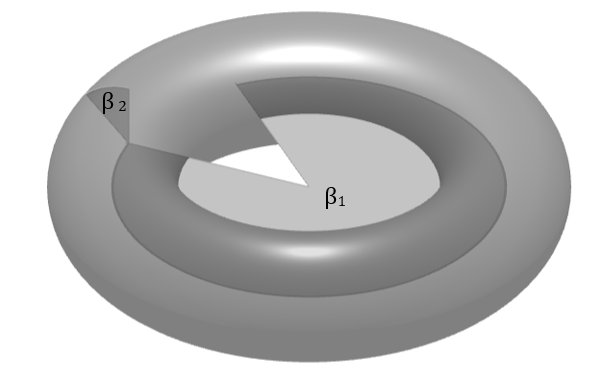
\includegraphics[scale=0.4]{./images/torus_labeled_angles.png}
\caption{Identifying the Positions on the Torus}
\label{fig:Torus Labeled Angles}
\end{figure}

\subsubsection{Demonstrating Homotopy}

Let $P_3$ be the Path graph with 3 edges and let $\ell: E(P_3) \rightarrow \mathbb R^+$ be arbitrary. Define a linkage $(P_3,\ell)$. This is our 2-arm, it has three links and the lengths can be anything as we have no cycles. We know our linkage is unrestricted, as it has no cycles, so consider:

$$M((P_3,\ell)) \simeq \{ \boldsymbol{\alpha} := (\alpha_1, \alpha_2) \, | \, \alpha_1, \alpha_2 \in \mathbb S^1 \}$$ 

\noindent We have two links, each can be positioned at any angle, hence a state of our linkage is given by $\boldsymbol{\alpha}$, a pair of angles. \\\\ Now consider the torus, any point on that manifold can be uniquely identified with two angles. Call these $\beta_1$ and $\beta_2$ (see figure \ref{fig:Torus Labeled Angles}), note this requires picking two positions to measure $\beta_1$ and $\beta_2$ against, but due to the symetries of the torus these are arbitrary. \\\\ Now to prove that the torus is homotopic to the configuration space of our 2-arm we need to find a pair of maps $f: M((P_3,\ell)) \rightarrow T^2 $ and $g: T^2 \rightarrow M((P_3,\ell))$ such that:

\begin{gather*}
f: M((P_3,\ell)) \rightarrow T^2 \\
g: T^2 \rightarrow M((P_3,\ell)) \\
s.t. f \, \circ g \simeq Id_{T^2} \, and \, g \, \circ f \simeq Id_{M((P_3,\ell))}
\end{gather*}

\noindent This is not hard, given the way we have set up the situation. Define $f$ as the map that takes the position of the linkage (given as ($\alpha_1, \alpha_2$)) to a position ($\beta_1$,$\beta_2$) on the torus. As in: 
\begin{gather*}
\forall \, (x_1, x_2) \in M((P_3,\ell)) \\ f((x_1,x_2)) = (x_1,x_2) \in T^2 \\\\
\forall \, (y_1, y_2) \in T^2 \\ g((y_1,y_2)) = (y_1,y_2) \in M((P_3, \ell))
\end{gather*}

\noindent Hence, take:

\begin{gather*}
(f \circ g)(y_1, y_2) = f((x_1,x_2)) = (y_1, y_2) \\
(g \circ f)(x_1, x_2) = f((y_1,y_2)) = (x_1, x_2)
\end{gather*}

\noindent Note, what we are doing here is using the homotopy: $M((P_3,\ell)) \simeq \mathbb S^1 \times \mathbb S^1 \simeq T^2$ by expressing the points in our configuration space and on the torus as points in $\mathbb S^1 \times \mathbb S^1$.

\section{Finding A Planar Linkage with a Given Configuration Space}
\subsection{Basic Idea}

We would like to be able to pick any 

% \section{Conclusion}

\bibliographystyle{plain}
\bibliography{references}
\end{document}